\documentclass[journal,onecolumn]{IEEEtran}
\usepackage[a5paper, margin=10mm]{geometry}
\usepackage{tfrupee}
\usepackage{booktabs}
\usepackage{graphicx} % For including figures
\usepackage{gvv-book}
\usepackage{gvv}


\begin{document}
	\title{
		%	\logo{
			\fontsize{18pt}{20pt}\selectfont Voltage-Temperature Calibration of PT-100 RTD using the Callendar-Van Dusen Equation and Noise Reduction using Random Forest Regression
			
			\large{EE1030 : Matrix Theory}
			
			Indian Institute of Technology Hyderabad
			%	}
	}
	\author{Yellanki Siddhanth
		
		(EE24BTECH11059)
	}	
	\maketitle
	\section{Objective}
	This experiment uses the Callendar-Van Dusen equation and the least squares method to model the relationship between temperature and voltage for a PT-100 RTD (Resistance Temperature Detector). The objective is to derive a polynomial calibration model that relates voltage output from the RTD to temperature, utilizing additional methods for improved fitting accuracy.
	\section{Procedure}
	\begin{enumerate}
		\item \textbf{Circuit Construction:} A circuit \ref{fig:circuit_diagram} was built on a breadboard to connect the PT-100 RTD sensor with the Arduino. The setup included necessary components such as resistors and a Wheatstone bridge for accurate voltage measurement. 
		
		\item \textbf{Temperature Measurement:} To validate the readings from the PT-100 RTD, an alcohol thermometer \ref{fig:alcohol_temperature} was used to measure the ambient temperature. Since reading can be difficult with an alcohol temperature \ref{fig:alcohol_temperature}, a digital temperature \ref{fig:digital_temperature} is a very good alternative for a reliable reference for comparison with the voltage output from the RTD sensor.
		
		\item \textbf{Data Collection:} The output voltages from the PT-100 RTD sensor were recorded at known temperature points using the Arduino, while simultaneously measuring the temperature with the alcohol thermometer. The temperature data was logged for further analysis. \textbf{Data Note:} To achieve a closer and more accurate plot, analog readings from the PT-100 RTD sensor were used instead of voltage readings. This approach allowed for greater precision in calibration. The relationship between voltage and analog readings is defined by \( V = k \times \text{Analog Readings} \), where \( k \) is a constant specific to the setup, which in the case of an arduino is $\frac{5}{1023}$.
		
	\end{enumerate}
	
	% Include images
	\begin{figure}[h]
		\centering
		\begin{minipage}[b]{0.45\textwidth}
			\centering
			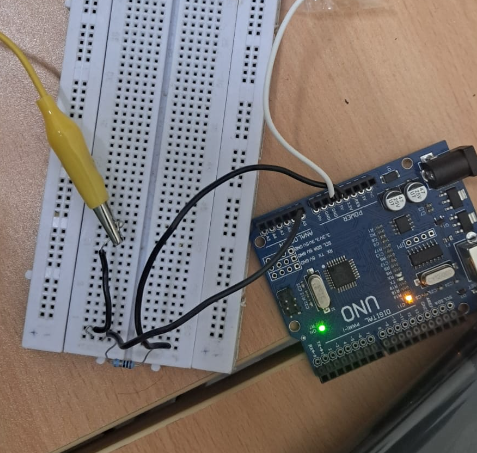
\includegraphics[width=\textwidth]{figs/circuit.png}
			\caption{Circuit for the PT-100 RTD setup.}
			\label{fig:circuit_diagram}
		\end{minipage}
		\hspace{0.05\textwidth}
		\begin{minipage}[b]{0.45\textwidth}
			\centering
			\begin{circuitikz} \draw
				(0,0) to[battery1, l=$5\ V$, invert] (0,2)
				to[R, l^=$10\ \Omega$] (3,2) to[short, -o] (5,2);
				\draw (3,2) to[R, l^=$P\ \Omega$] (3,0)
				-- (0,0);
				\draw (3,0) to[short, -o] (5,0);
			\end{circuitikz}
			\caption{Schematic Circuit Diagram to Measure the Output of PT-100.}
			\label{fig:ckt}
		\end{minipage}
	\end{figure}
		\begin{figure}[h]
		\centering
		\begin{minipage}[b]{0.45\textwidth}
			\centering
			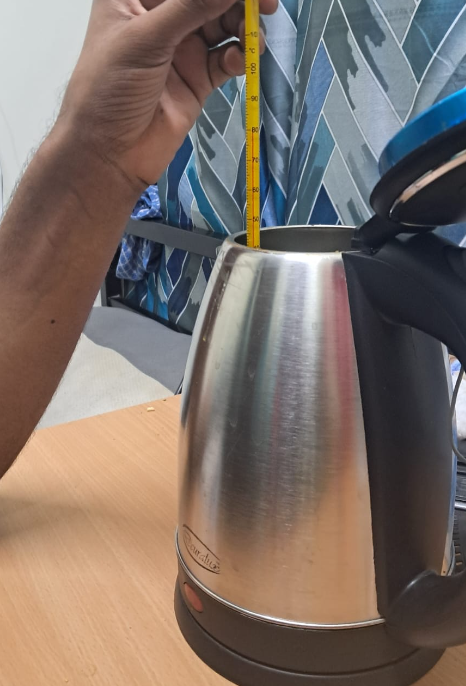
\includegraphics[width=0.45\textwidth]{figs/alcohol.png}
			\caption{Temperature measuring setup using an alcohol thermometer.}
			\label{fig:alcohol_temperature}
		\end{minipage}
		\hspace{0.05\textwidth}
		\begin{minipage}[b]{0.45\textwidth}
				\centering
				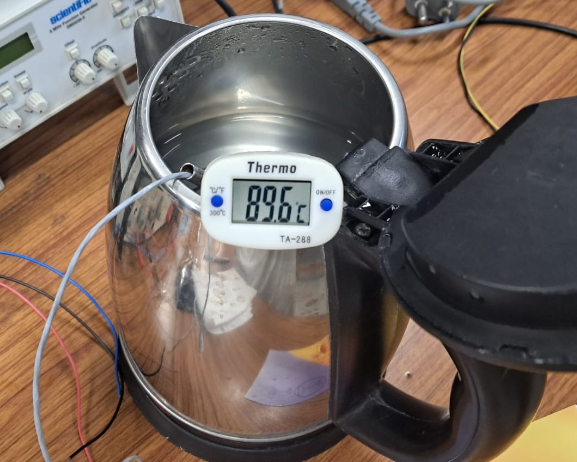
\includegraphics[width=0.8\textwidth]{figs/digital.png}
				\caption{Temperature measuring setup using a digital thermometer.}
				\label{fig:digital_temperature}
		\end{minipage}
	\end{figure}
	\section{Training Data}
	The training data collected by the PT-100 RTD sensor, as measured by an Arduino, are presented in Table \ref{tab:training_data}. This data will be used to fit the Callendar-Van Dusen model to describe the voltage-temperature relationship.
	
	\begin{table}[h]
		\centering
		\begin{minipage}[b]{0.45\textwidth}
			\centering
			\caption{Training data for PT-100 calibration.}
			\label{tab:training_data}
			\begin{tabular}{@{}cc@{}}
				\toprule
				Temperature (°C) & Analog Input (A0) \\ \midrule
				73.0                 & 953         \\
				46.8                 & 948         \\
				40.8                 & 947         \\
				54.5                 & 949         \\
				59.4                 & 950         \\
				56.5                 & 950         \\
				50.4                 & 949         \\
				36.0                 & 946         \\
				61.8                 & 951         \\
				91.2                 & 956         \\
				96.1                 & 957         \\
				89.4                 & 956         \\
				33.8                 & 945         \\
				86.3                 & 955         \\
				28.4                 & 944         \\
				83.9                 & 955         \\
				67.2                 & 952         \\
				64.5                 & 951         \\
				44.9                 & 947         \\ \bottomrule
			\end{tabular}
		\end{minipage}
		\hspace{0.009\textwidth}
		\begin{minipage}[b]{0.45\textwidth}
			\centering
			\caption{Denoised training data for PT-100 calibration.}
			\label{tab:denoised_training_data}
			\begin{tabular}{@{}cc@{}}
				\toprule
				Denoised Temperature (°C) & Analog Input (A0) \\ \midrule
				70.72531286              & 953        \\
				45.85104667              & 948        \\
				42.50149357              & 947        \\
				52.20067667              & 949        \\
				57.41318143              & 950        \\
				57.41318143              & 950        \\
				52.20067667              & 949        \\
				36.08730167              & 946        \\
				62.59749571              & 951        \\
				89.68815429              & 956        \\
				93.74424429              & 957        \\
				89.68815429              & 956        \\
				33.07323                 & 945        \\
				85.60526857              & 955        \\
				30.98883                 & 944        \\
				85.60526857              & 955        \\
				65.92970619              & 952        \\
				62.59749571              & 951        \\
				42.50149357              & 947        \\ \bottomrule
			\end{tabular}
		\end{minipage}
	\end{table}
	
	
	% Add the Training Fit Image
	\section{Results from Least Squares Method}
	The regression yielded the following model:
	\begin{equation}
		V(T) = V(0) \left( 1 + AT + BT^2 \right)
	\end{equation}
	with coefficients:
	\begin{itemize}
		\item \( V(0) \approx \text{4.578899430486582} \)
		\item \( A \approx \text{0.0002800324245079253} \)
		\item \( B \approx \text{-5.81408492749038e-07} \)
	\end{itemize}
	
	% Include Training Fit Image
	\begin{figure}[h]
		\centering
		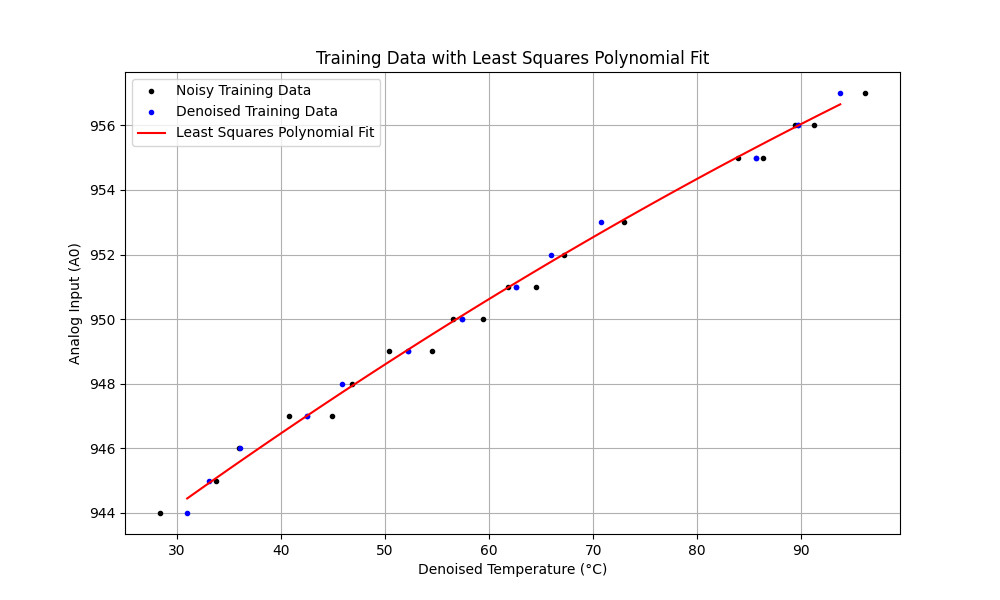
\includegraphics[width=1\textwidth]{figs/train_fit.png}
		\caption{Training data with least squares polynomial fit.}
		\label{fig:train_fit}
	\end{figure}
	
	\section{Random Forest Regressor}
	To improve the fit of the polynomial model, a Random Forest Regressor was employed. This ensemble learning method constructs multiple decision trees during training and outputs the mean prediction of individual trees.
	
	\begin{enumerate}
		\item \textbf{Training:} The training data was used to fit the Random Forest model, which captures complex relationships between the input features (temperature) and the target variable (voltage).
		
		\item \textbf{Prediction:} The Random Forest model provides a flexible approach, accommodating non-linear relationships without requiring explicit polynomial terms.
		
		The predicted voltage values \ref{tab:denoised_training_data} from the Random Forest model were then compared against the measured voltages, demonstrating improved accuracy in fitting.
	\end{enumerate}
	\section{Validation}
	To validate the models, additional temperature points were used. The measured voltage values were compared to those predicted by the models, as shown in Table \ref{tab:validation_data}.
		\begin{table}[h]
		\centering
		\begin{minipage}[b]{0.45\textwidth}
			\centering
					\caption{Measured validation data.}
			\label{tab:validation_data}
			\begin{tabular}{@{}cc@{}}
				\toprule
				Temperature (°C) & Analog Input (A0) \\ \midrule
				69.1                 & 952          \\
				80.7                 & 954          \\
				48.6                 & 948          \\
				63.6                 & 951          \\
				38.4                 & 946          \\
				50.6                 & 949          \\
				95.5                 & 957          \\
				58.1                 & 950          \\ \bottomrule
			\end{tabular}
		\end{minipage}
		\hspace{0.009\textwidth}
		\begin{minipage}[b]{0.45\textwidth}
			\centering
					\caption{Denoised validation data.}
			\label{tab:denoised_validation_data}
			\begin{tabular}{@{}cc@{}}
				\toprule
				Temperature (°C) & Analog Input (A0) \\ \midrule
				65.92970619                 & 952          \\
				76.95450857                 & 954          \\
				45.85104667                 & 948          \\
				62.59749571                 & 951          \\
				36.08730167                 & 946          \\
				52.20067667                 & 949          \\
				93.74424429                 & 957          \\
				57.41318143                 & 950          \\ \bottomrule
			\end{tabular}
		\end{minipage}
	\end{table}

	% Include Validation Fit Image
	\begin{figure}[h]
		\centering
		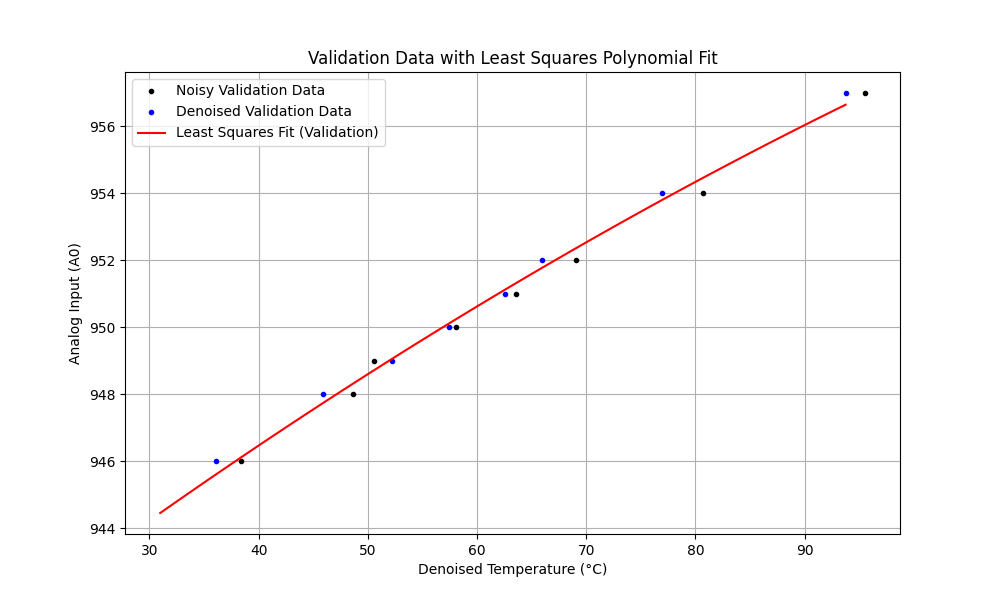
\includegraphics[width=1\textwidth]{figs/valid_fit.png}
		\caption{Validation data with least squares polynomial fit.}
		\label{fig:valid_fit}
	\end{figure}
	\section{Conclusion}
	The derived models accurately capture the relationship between voltage and temperature for the PT-100 RTD, allowing the Arduino to estimate temperature from voltage measurements over the calibrated range. The Random Forest Regressor provided improved fits, demonstrating their utility alongside traditional least squares methods.
	
	\section{Code}
	The calibration and regression processes were controlled using the C++ source file \texttt{codes/data.cpp}, which was uploaded to the Arduino using PlatformIO. The Random Forest regression was implemented using the \texttt{scikit-learn} library in Python, which provides an efficient way to fit ensemble learning models and improve prediction accuracy. The plotting and least square computation python file can be referred from \texttt{codes/lsqn.py}
	
	
\end{document}
